\documentclass[english,12pt]{article}

\usepackage{amsthm}
\usepackage[latin9]{inputenc}
\usepackage{babel}
\usepackage[hmargin=0.9in,vmargin=1.25in]{geometry}
\usepackage{graphicx}
\usepackage{subfigure}
\usepackage[colorlinks=true,citecolor=blue,urlcolor=blue]{hyperref}
\usepackage{amsmath}
\usepackage{amssymb,amsfonts}

\newtheorem{thm}{Theorem}
\newtheorem{lem}{Lemma}
\newtheorem{cor}{Corollary}
\newtheorem{dfn}{Definition}

\newcommand{\Rnot}{\sigma_0}
\newcommand{\Sinf}{x_\infty}
\newcommand{\dom}{{\mathcal D}}
\newcommand{\R}{{\mathbb R}}
\newcommand{\xopt}{x_\text{opt}}
\newcommand{\yopt}{y_\text{opt}}

\DeclareMathOperator\supp{supp}

\begin{document}
\title{Optimal control of an SIR epidemic through finite-time non-pharmaceutical intervention}
\author{
  David I. Ketcheson\thanks{Computer, Electrical, and Mathematical Sciences \& Engineering Division,
King Abdullah University of Science and Technology, 4700 KAUST, Thuwal
23955, Saudi Arabia. (david.ketcheson@kaust.edu.sa)}
}
\maketitle

\abstract{We consider the problem of controlling an epidemic within the SIR
framework by temporarily reducing the rate of contact within a population.
The control takes the form of a multiplicative reduction in the contact rate
of infectious individuals.  The control is allowed to be applied only over
a finite time interval, while the objective is to minimize the total number of
individuals infected in the long-time limit, subject to some cost function for
the control.  We first consider the no-cost scenario and analytically determine
the optimal control and solution.  Various other cost functions are considered
and optimal solutions given analytically or computed for each.
}

\section{Problem description and assumptions}
The classical SIR model of Kermack \& Mckendrick \cite{kermack1927contribution} is
\begin{subequations} \label{SIR}
\begin{align} 
    x'(t) & = -\beta y(t) x(t) \label{eq:x} \\
    y'(t) & = \beta y(t) x(t) - \gamma y(t) \label{eq:y} \\
    (x(0),y(0)) & \in \dom := \{(x_0,y_0) : x_0 \ge 0, y_0\ge 0, x_0+y_0 \le 1\},
\end{align}
\end{subequations}
where $x(t), y(t)$ represent the susceptible and infected populations
respectively, while the recovered population is $z(t)=1-x(t)-y(t)$.  The region
$\dom$ is forward-invariant and a unique solution exists for all time
\cite{hethcote2000mathematics}.  While
the temporal dynamics of \eqref{SIR} depend on both $\beta$ and $\gamma$, the set
of trajectories depends only on the basic reproduction number 
$\Rnot = \beta/\gamma$.  Dynamics for two values of $\Rnot$ are
shown in Figure \ref{fig:dynamics}.  The system
is at equilibrium if $y(t)=0$.  This equilibrium is stable if and
only if $x(t)\le 1/\Rnot$, a condition referred to as {\em herd immunity}.  If
this condition is not satisfied at
the initial time, then $y(t)$ will first increase until it is, and then decrease,
approaching zero asymptotically.  The SIR model assumes that recovery
confers permanent immunity.

\begin{figure}
    \centering
    \subfigure[$\sigma=3$]{\label{sigma3}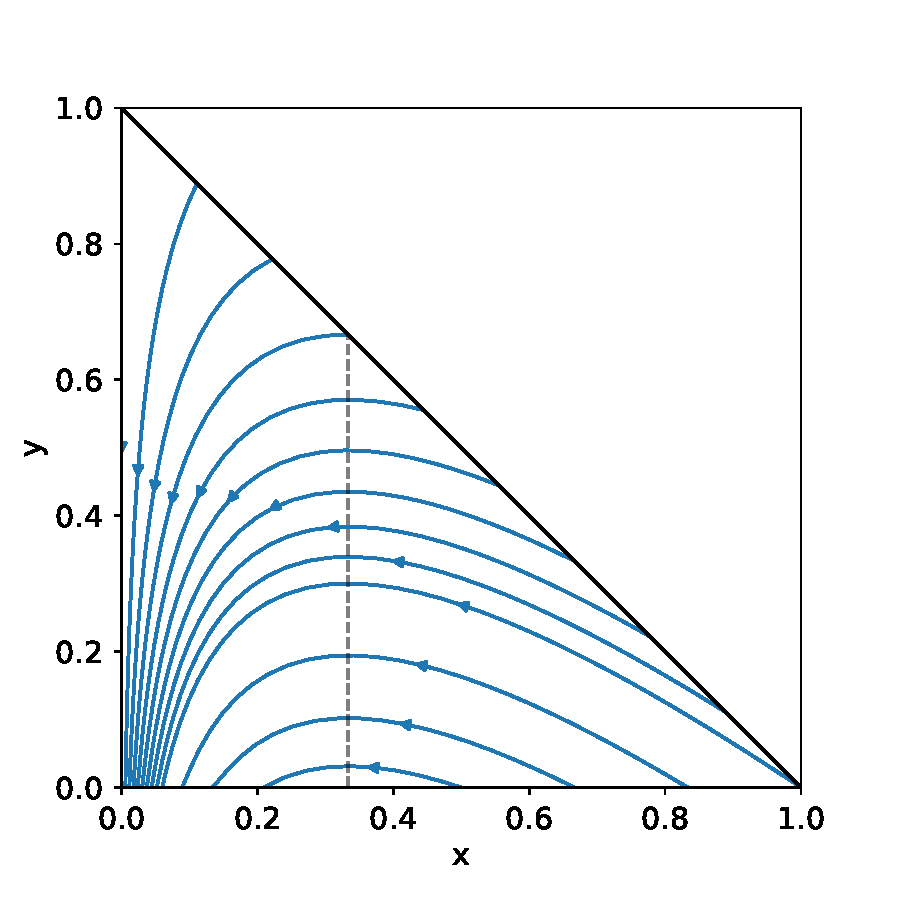
\includegraphics[width=0.49\textwidth]{figures/sigma3.pdf}}
    \subfigure[$\sigma=1.5$]{\label{sigma15}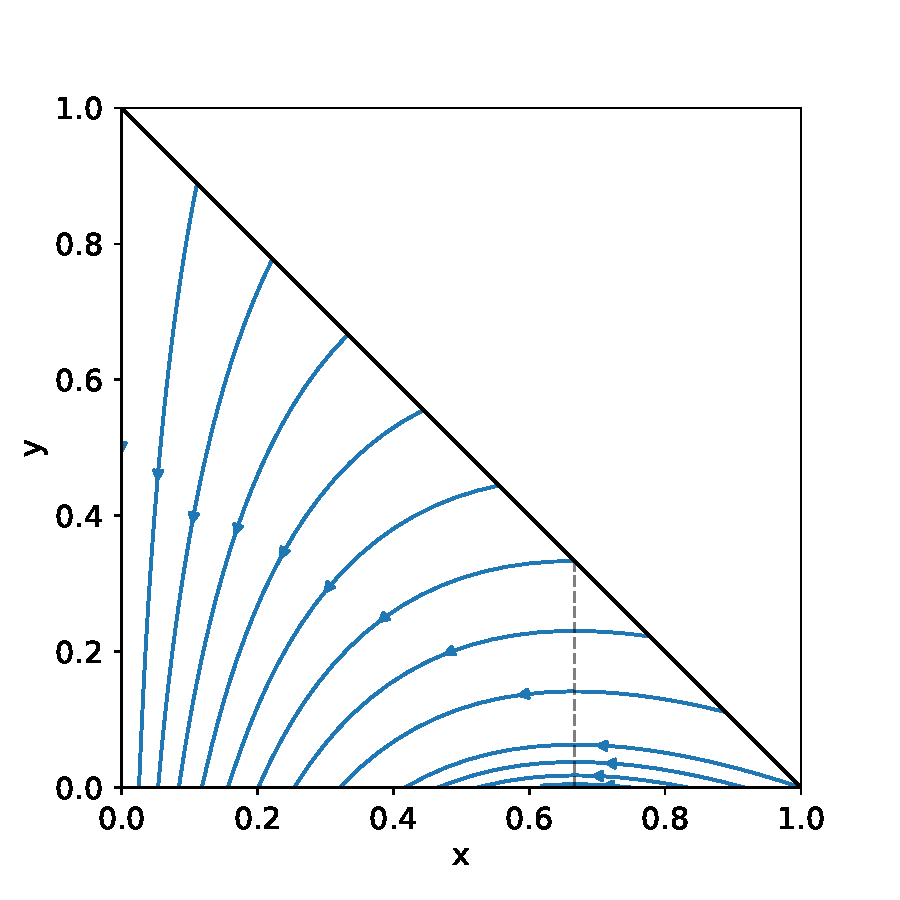
\includegraphics[width=0.49\textwidth]{figures/sigma15.pdf}}
    \caption{Dynamics of SIR model for two values of the basic reproduction number.
            The critical value $x=1/\sigma$ is shown with a dashed line.\label{fig:dynamics}}
\end{figure}

For many diseases affecting humans, herd immunity is achieved
through vaccination of a sufficient portion of the population.  Herein
we assume a vaccine is unavailable, so that herd immunity can only be achieved
through infection and recovery.
Our goal is to minimize $z_\infty := \lim_{t \to \infty} z(t)$, or equivalently
(since $y_\infty=0$)
to maximize the long-time limit of the susceptible fraction:
\begin{align}
    \Sinf = \lim_{t\to\infty} x(t).
\end{align}
This has the effect of minimizing
the number of eventual deaths, which would be proportional to $z_\infty$.

This is equivalent to minimizing the number of deaths, if we assume that
some fraction of the recovered population $z(t)$ dies from the disease.
From the foregoing it is clear that $\Sinf \le 1/\Rnot$.  The difference
$\Rnot-\Sinf$ is referred to as {\em epidemiological overshoot}.

This overshoot can in principle be reduced through so-called
non-pharmaceutical intervention (NPI), which is simply a means to
reduce contact between infected and susceptible individuals.  We model a NPI
control via a time-dependent parameter $q(t)\in[0,1]$ with the SIRq system
\begin{subequations} \label{SIRq}
\begin{align}
    x'(t) & = -(1-q(t))\beta y x \\
    y'(t) & = (1-q(t))\beta y x - \gamma y.
\end{align}
\end{subequations}
An active control $q(t)>0$ reduces the effective reproduction number which is now
given by $\sigma(t) = (1-q(t))\Rnot$.  This can account for both
population-wide interventions and interventions specific to identified infectious
(or possibly infectious) individuals.  

Most epidemics do not result in substantial permanent changes in the contact rate of
a population.  We therefore assume 
\begin{align} \label{q-shortterm}
    q(t)=0 \text{ for } t>T,
\end{align}
i.e., that intervention can only be applied over a limited time, up to $T$.
Since $x_\infty=1/\sigma_0$ only at the single point $(x=1/\sigma_0,y=0)$, and since 
the $y=0$ axis cannot be reached in a finite time, we know that any solution
must have $x_\infty<1/\sigma_0$.
%In either model \eqref{SIR} or \eqref{SIRq}, the zero-infection axis
%$y=0$ can only be reached after an infinite amount of time. Therefore our
%objective will be to achieve $x_\infty=1/\sigma_0 - \epsilon$ for a prescribed
%value $\epsilon$.

We state the control problem as follows:
\begin{align} \label{eq:basic-problem}
\begin{aligned}
& \text{Given } x_0, y_0, \sigma_0, T, \text{ choose } q(t) \in [0,1] \text{ to minimize }  \\
&     J = -x_\infty(x(T),y(T),\sigma_0) + c_2 \int_0^T f(q(t) dt \\
& \text{ subject to } \eqref{SIRq}.
\end{aligned}
\end{align}
Here $J(x_\infty,q)$ is the objective function that accounts for the desire to
minimize infections as well as a cost of imposing control.


\subsection{Related Work}
Optimal control in the SIR model with vaccination has been studied in \cite{kar2011stability}.
Optimal control for an extended SIR model, based on quarantining and isolation
of confirmed or suspected cases was studied in \cite{yan2008optimal}.  
A review of work on optimal control in epidemiology is presented in \cite{sharomi2017optimal},
along with the formulation of the optimal control solution (based on
Pontryagin's maximum principle) for several extensions of the SIR model.

The present work differs from those referenced above in multiple important
respects.  First, in order to gain general insight rather than disease-specific
results, we focus on analytical rather than computational solutions.  Most solutions
are derived directly rather than (as is most commonly done) via Pontryagin's maximum principle.
Second, we assume that no vaccine is available.  Third, we seek a control that is optimal
in terms of the asymptotic cumulative number of infected, while also considering the
situation in which the control cannot be applied only over a finite time.

\subsection{Outline}
The rest of the paper is organized as follows.  In Section \ref{sec:prelims} we
review results on the exact solution of the SIR model and compute some quantities
that will be central to our results.  In Section \ref{sec:analytic} we state
and prove solutions of \eqref{eq:basic-problem} under certain choices of $J$.
In Section X we illustrate results for other choices of $J$ with computational
examples.

\section{Preliminaries\label{sec:prelims}}

\subsection{Notation}
The control above is given as $q(t)$, but for most purposes it is more
convenient to work with the effective reproduction number, defined as
$$
    \sigma(t) := (1-q(t))\Rnot = (1-q(t))\beta/\gamma.
$$
We will often simply refer to $\sigma(t)$ as the control.

In general, the solution of \eqref{SIRq} depends on the initial data
$(x_0,y_0)$, the control $\sigma(t)$, and time $t$, so it is natural to write
$x(t;\sigma(t),x_0,y_0)$.
In what follows it will be convenient to make a slight abuse of notation and
write $x(t;\sigma(t))$ or $x(t)$ when there is no chance of confusion.

For a fixed reproduction number, the asymptotic susceptible fraction $\Sinf$
can be obtained from the solution $x(t), y(t)$ at any time $t$, since solutions
of \eqref{SIR} move along contours of $\Sinf$.  Thus we will write $\Sinf(x,y)$
or $\Sinf(x,y,\Rnot)$.

\begin{dfn} ({\bf Admissible control})
Given a basic reproduction number $\Rnot$, we say a control fuction $\sigma(t)$ is
admissible if $0\le \sigma(t) \le \sigma_0$ for all $t$.
\end{dfn}

\subsection{Solutions of the basic SIR model}
Here we review results on the solution of \eqref{SIR}.
It is straightforward to show that $x(t)$ satisfies (see e.g.
\cite{harko2014exact,pakes2015lambert})
$$
    x(t) = x_0 e^{\Rnot(z_0-z(t))}.
$$
Since $z=1-x-y$ we find that
$$
   \mu(x_0,y_0,\Rnot) := x_0 e^{-\Rnot(x_0+y_0)} =  x(t) e^{-\Rnot(x(t)+y(t))} 
$$
In other words, $\mu$ is constant in time, and the trajectories
in Figure \ref{fig:dynamics} are contours of $\mu$.
Since also $y_\infty=0$, we have
$$
    x_\infty = x_0 e^{\Rnot(x_\infty-x_0-y_0)} = \mu(x_0,y_0,\Rnot) e^{\Rnot x_\infty}.
$$
Setting $w=-x_\infty \Rnot$ we have
$$
    we^w = -x_0 \Rnot e^{-\Rnot(x_0+y_0)} = -\mu \Rnot.
$$
Thus $w = W_0(-\mu\Rnot)$ where $W_0$ is the principal branch of Lambert's $W$-function \cite{pakes2015lambert},
and
$$
    x_\infty = -\frac{1}{\Rnot}W_0(-\mu \Rnot).
$$
In what follows we will make use of the derivatives of $\Sinf$ with respect to $x$ and $y$.
We have
\begin{align*}
\frac{d \Sinf}{d\mu} = W'(-\mu \Rnot) = \frac{1}{e^{-\Rnot\Sinf}-\mu \Rnot} > 0,
\end{align*}
so $\Sinf$ is a monotone function of $\mu$ and maximizing the former is equivalent to
maximizing the latter.
Now
\begin{align*}
    \frac{d}{dt} \mu(x(t;\sigma(t)),y(t;\sigma(t)),\Rnot) = (\Rnot-\sigma(t))\gamma y(t;\sigma(t)) \mu(t).
\end{align*}
\begin{align*}
    \frac{\partial \Sinf}{\partial y} & = W'(-\mu\Rnot) \frac{\partial \mu}{\partial y}
\end{align*}


The formulas in this section also hold for the solution of \eqref{SIRq} if
$q(t)$ is a constant function and $\Rnot$ is replaced in these formulas by
$\sigma=(1-q)\Rnot$.


%We define the solution operator $\phi_t(\beta,\gamma): \dom \to \dom$ as the map
%that takes an initial condition $(x_0,y_0)$ to the solution $(x(t),y(t))$
%via the solution of \eqref{SIR}.  We further define for $u\in\dom$
%$$
%    x_\infty(u,\sigma) = \lim_{t\to\infty} \phi_t(\sigma,1)u.
%$$
%Observe that each trajectory in Figure \ref{fig:dynamics} is a contour of $x_\infty$.
%Our objective then is to minimize $x_\infty((x(T),y(T)),\Rnot)$.

(need to show that $\Sinf$ is a decreasing function of $y$ before this lemma)

By applying the control we can move the solution to a different contour of
$x_\infty(\cdot,\sigma)$.  The next lemma states that applying any control $q>0$ over
any length of time leads to an increase in $x_\infty$.
\begin{lem}
Let $\Rnot>0$ and $u\in\dom$ be given and define $X_\infty = x_\infty(x_0,y_0,\Rnot)$.
Let $\sigma(t)$ be an admissible control such that $\sigma(t)<\sigma_0$ over some
half-open set $t\in[0,\epsilon)$.  Then for any $t>0$ we have
$$
    x_\infty(x(t;\sigma(t)),y(t;\sigma(t)),\Rnot) > X_\infty.
$$
\end{lem}
\begin{proof}
    Dividing \eqref{eq:y} by \eqref{eq:x} gives
    \begin{align} \label{eq:dydx}
        \frac{dy}{dx} = -1 + \frac{1}{\sigma x}.
    \end{align}
    Thus reducing $\sigma$ has the effect of increasing $dy/dx$.
    Since all trajectories flow to the left ($x$ is a decreasing function of $t$),
    this means that the solution trajectory obtained with $\sigma(t)$ lies
    below that obtained with $\sigma_0$, for all $t>0$.
\end{proof}

%\begin{cor} \label{cor:diff-control}
%Let two control functions $q(t), \hat{q}(t)$ be given with $\hat{q}(t)<q(t)$.
%Then $x_\infty(q)>x_\infty(\hat{q})$.
%\end{cor}

In the classic SIR model, the asymptotic susceptible fraction $\Sinf$ is
given as a function of the initial state and of $\Rnot$ by the unique solution 
in the interval $(0,1/\Rnot)$ of the
following equation \cite[Eqn. (5.4)]{hethcote1989three}:
\begin{align} \label{s-infty}
    1 - z_0 - \Sinf + \frac{1}{\Rnot} \log\left(\frac{\Sinf}{x_0}\right) = 0.
\end{align}

\begin{thm}
Let $y_0>0$ and
let $\Sinf(q) = \lim_{t\to\infty} x(t;q)$ where $x(t;q)$ denotes the solution of
\eqref{SIRq} subject to \eqref{q-shortterm}.  Then $\Sinf\le 1/\sigma$.
\end{thm}
\begin{proof}
Due to condition \eqref{q-shortterm}, as $t \to \infty$ the solution of \eqref{SIRq}
must tend to a stable equilibrium point of \eqref{SIR}.  But the stable equilibrium
points of \eqref{SIR} satisfy $x \le 1/\sigma$.
\end{proof}

\subsection{Formulation as a boundary value problem}
Standard application of Pontryagin's maximum principle gives necessary conditions
for a solution of \eqref{eq:basic-problem}.  The Hamiltonian for this problem is
$$
    H(t) = -\lambda_1(t) \gamma \sigma(t) y(t) x(t) + \lambda_2(t)\gamma y(t)(\sigma(t) x(t) - 1) + c_2 f(q).
$$
The Pontryagin maximum priniciple gives necessary conditions for an optimal control, which consist of $\eqref{SIRq}$
together with
\begin{subequations}\label{lambda-odes}
\begin{align} 
    \lambda_1'(t) & = (\lambda_1-\lambda_2)\gamma\sigma(t) y \\
    \lambda_2'(t) & = (\lambda_1-\lambda_2)\gamma\sigma(t) x + \lambda_2 \gamma \\
    \lambda_2(T) & = \frac{\partial }{\partial y(T)} (-x_\infty(x(T),y(T),\sigma_0) \\
    \lambda_1(T) & = \frac{\partial }{\partial x(T)} (-x_\infty(x(T),y(T),\sigma_0) = \left(1-\frac{1}{x(T)\sigma_0}\right)\lambda_2(T),
\end{align}
\end{subequations}
as well as the condition $\partial H/\partial \sigma = 0$, which reads
\begin{align*}
    \sigma(t) = \sigma_0 + \frac{(\lambda_2(t)-\lambda_1(t))\gamma y x}{2c_2},
\end{align*}
in addition to which we impose the the constraint $0\le \sigma(t) \le \sigma_0$, yielding
\begin{align} \label{eq:sigma-c2}
    \sigma(t) = \max\left(0,\min\left(\sigma_0,\sigma_0 + \frac{\lambda_2(t)-\lambda_1(t))\gamma y x}{2c_2}\right)\right).
\end{align}

\section{Analytic optimal controls\label{sec:analytic}}
%No trajectory starting from $y_0>0$ reaches $y(t)=0$ in finite time, regardless of the
%value of $\sigma$.  Hence it is impossible to reach the optimal equilibrium state
%$(1/\sigma_0,0)$ with a finite-time control.  Therefore we look for $\epsilon$-optimal
%solutions that tend to an equilibrium $(x_\infty,0)$ with $x_\infty > 1/\sigma_0 - \epsilon$.

\subsection{Zero-cost, finite time control}
We start by investigating the control problem \eqref{eq:basic-problem} when the control
can be applied at no cost (equivalently, when the goal of increasing $x_\infty$ completely
trumps any associated costs).  This is given by taking $c_2 = 0$ in \eqref{eq:basic-problem}:
\begin{align} \label{eq:no-cost-problem}
\begin{aligned}
& \text{Given } x_0, y_0, \sigma_0, T, \text{ choose } q(t) \in [0,1] \\
& \text{ to minimize }  J = -x_\infty(x(T),y(T),\sigma_0) \\
& \text{ subject to } \eqref{SIRq}.
\end{aligned}
\end{align}

\begin{thm}
An optimal control for \eqref{eq:no-cost-problem} is given by
\begin{align}
    q(t) & = \begin{cases}  
        0 & t<t^* \\
        1 & t^* \le  t \le T,
    \end{cases}
\end{align}
where $t^*=0$ if $x(0)\le1/\sigma_0$ and otherwise $t^*$ is the unique solution of
\begin{align} \label{xtstar}
    x(t^*;\Rnot,x_0,y_0) = \frac{1}{\sigma_0(1-e^{-\gamma(T-t^*)})}.
\end{align}
\end{thm}
\begin{proof}
First, suppose $x(0)\le1/\sigma_0$.  The claimed optimal control gives $x(T)=x_0$, whereas
any other control will give $x(T)<x_0$.  Similarly, we see from \eqref{SIRq} that
the optimal control gives $y(T)=e^{-\gamma T}y_0$ and any other control will
lead to a larger value of $y(T)$.  Since $\Sinf$ is a decreasing function of $y$ and
(for $x<1/\Rnot$) an increasing function of $x$, the proposed control is optimal in this case.

Now suppose $x(0)>1/\sigma_0$.  Taking the limit $c_2\to 0$ in \eqref{eq:sigma-c2} gives
\begin{align}
    \sigma(t) & = \begin{cases} 0 & \lambda_1(t)>\lambda_2(t) \\ \sigma_0 & \lambda_1(t) < \lambda_2(t). \end{cases}
\end{align}
In other words, the solution is a bang-bang control that switches when $\lambda_2-\lambda_1$ changes sign.
Since $\lambda_2(T)<\lambda_1(T)<0$, we have $\sigma(T)=0$.  We can integrate \eqref{lambda-odes} backward from the final
time with $\sigma=0$ to find when $\lambda_1=\lambda_2$.  This yields \eqref{xtstar}.

It remains to show that the optimal control for $t<t^*$ is given by $q=0$.  
Let $(\xopt,\yopt)$ denote the optimal solution at time $T$.  There cannot be a
control that gives $(x(t^*),y(t^*)) = (\xopt,\yopt)$ for some $t^*<T$, since then
we could obtain a better solution by using that control combined with the choice
$q(t)=1$ for $t>t^*$.  In other words,
the optimal control is the one that arrives at $(\xopt,\yopt)$ in the shortest time,
starting from $(x_0,y_0)$.  The result then follows from Lemma \ref{lem:shortest-path}.
\end{proof}

\begin{lem} \label{lem:shortest-path}
Let $(x_0,y_0)$ and $(x_1,y_1)$ be given such that $x_0, x_1 \ge 1/\Rnot$ and
$\Sinf(x_0,y_0,\Rnot)\ge\Sinf(x_1,y_1,\Rnot)$.
Let $q(t)$ be a bang-bang control such that $(x(t_1;x_0,y_0,\sigma(t)),y(t_1;x_0,y_0,\sigma(t)))=(x_1,y_1)$
for some $t_1\ge0$.  Then the minimum value of $t_1$ is achieved by taking
\begin{align}
    q(t) & = \begin{cases}  
        0 & t<t^* \\
        1 & t^* \le  t \le T,
    \end{cases}
\end{align}
where $t^*$ satisfies $x(t^*;x_0,y_0,\Rnot)=x_1$.
\end{lem}
\begin{proof}
Since $q(t)$ is a bang-bang control, the trajectory $(x(t;q(t)),y(t;q(t)))$ 
consists of a sequence of segments each of which is a solution of
\eqref{SIRq} with $\sigma=0$ (traveling directly downward) or with $\sigma=\sigma_0$
(traveling along a contour of $x_\infty$).  Some trajectories of this type are
illustrated in Figure \ref{fig:bangbangtraj}.  Notice that each trajectory must
traverse the same distance in the x-direction; since $x'(t)=-\beta xy$ this
travel is faster at larger $y$ values.  Meanwhile, the total length of all the
downward ($\sigma=0$) segments is the same for any trajectory, and since for
these segments $y'(t) = -\gamma y$, travel is again faster at larger $y$ values.
The control given in the lemma makes all these traversals at the largest
possible value of $y$, so it arrives in the shortest time.
\end{proof}
The lemma above holds for the set of all admissible controls, but here we
only need the result for bang-bang controls.

\begin{figure}
    \centering
    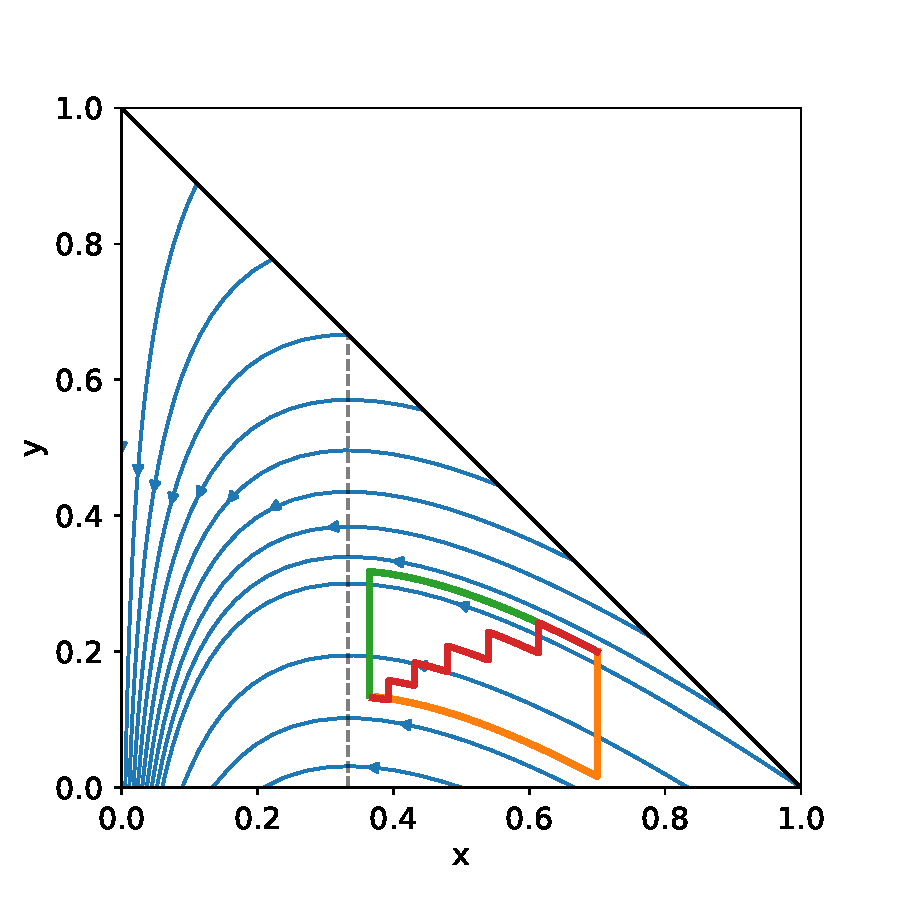
\includegraphics[width=0.5\textwidth]{figures/threepaths.pdf}
    \caption{Three different paths between two states, each obtained
    with a bang-bang control.  The top (green) path arrives in the shortest time.\label{fig:bangbangtraj}}
\end{figure}

\begin{figure}
    \centering
    \subfigure[Solution and control vs. time]{\label{fig:ex1-time}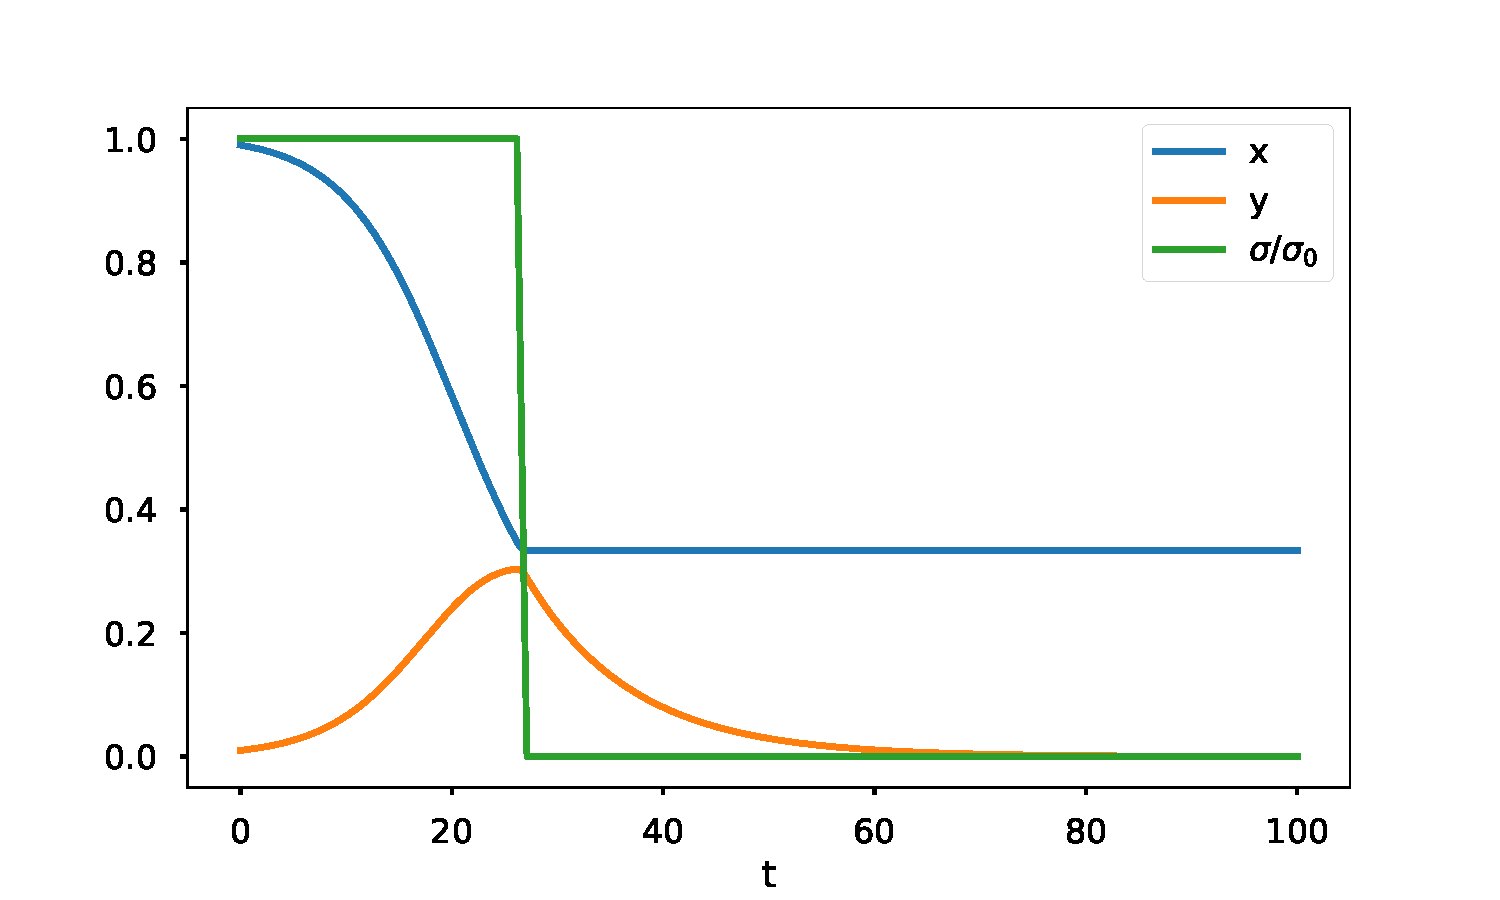
\includegraphics[width=0.65\textwidth]{figures/example1_time.pdf}}
    \subfigure[Trajectory in phase space]{\label{fig:ex1-xy}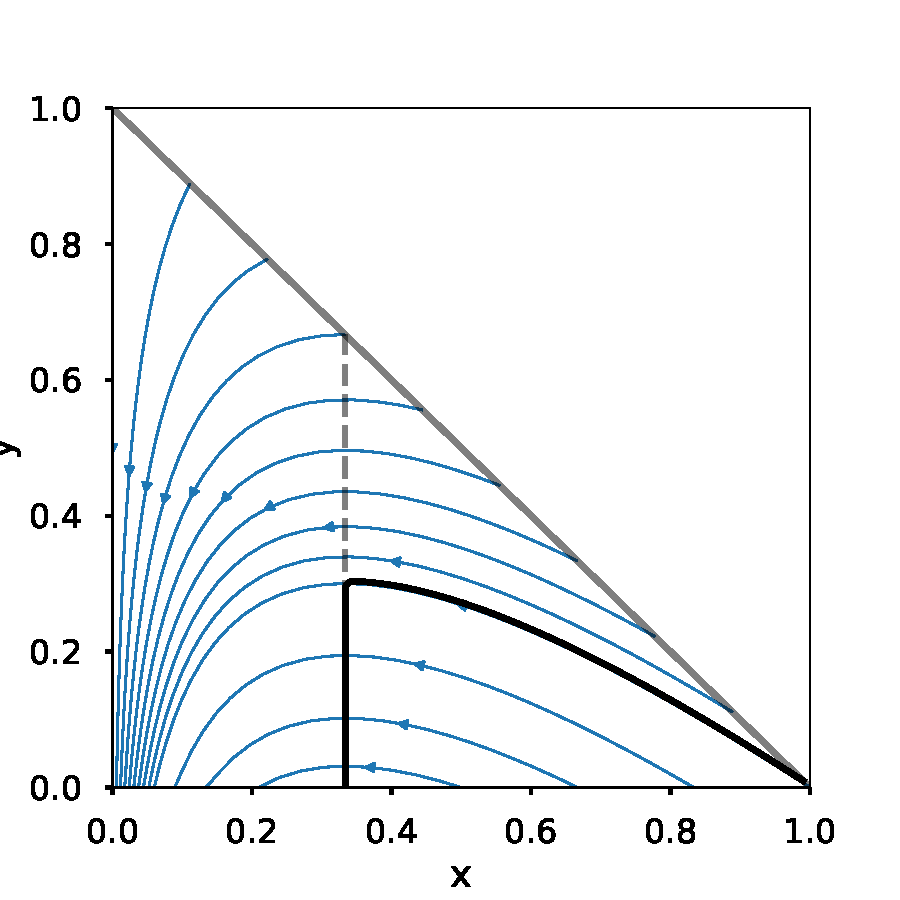
\includegraphics[width=0.34\textwidth]{figures/example1_xy.pdf}}
    \caption{Typical Pareto-optimal solution.  Here $(x(0),y(0)) = (0.99,0.01)$, $\beta=0.3$, and $\gamma=0.1$.\label{fig:example1}}
\end{figure}

\subsection{Max-norm cost, infinite-time control}
If the control can be applied over a semi-infinite time interval, there are many ways
to achieve the optimal value $\Sinf = 1/\Rnot$.  A natural question is, what is the
minimum of the maximum control that can be employed to reach this optimum?  We formulate
the problem as follows:
\begin{align} \label{eq:max-inf-problem}
\begin{aligned}
& \text{Given } x_0, y_0, \sigma_0, \text{ choose } q(t) \in [0,1] \text{ to minimize }  \\
&     J = -\lim_{t\to\infty} x(t) + c_2 \max_t q(t) \\
& \text{ subject to } \eqref{SIRq}.
\end{aligned}
\end{align}
For any finite $c_2$, the problem has a unique solution, even though in the limit
it does not.

\begin{thm}
In the limit $c_2 \to 0$, the unique optimal control for \eqref{eq:max-inf-problem} tends to
$$
    q(t) = 1-\frac{\sigma_*}{\sigma}
$$
where
$$
    -\frac{1}{\sigma_*} W_0(-\mu(x_0,y_0,\sigma_*)\sigma_*) = \frac{1}{\sigma_0}.
$$
\end{thm}
\begin{proof}
    The optimality of the given control follows from the fact that $\Sinf \le 1/\Rnot$ and
    that with this control we attain this bound.  To see the uniqueness, observe that
    \eqref{eq:dydx} implies that imposing a larger value of $\sigma$ at any time will lead
    to a solution that lies above the optimal trajectory, and therefore must terminate at
    a smaller $\Sinf$.
\end{proof}

\subsection{Minimization of the maximum control}
\begin{align} \label{eq:minmax}
\text{Given } x_0, y_0, \sigma_0, \text{ minimize } \max_t(q(t)) \text{ subject to } \eqref{SIRq} \text{ and } \lim_{t\to\infty} x(t) = \frac{1}{\sigma}.
\end{align}
\begin{thm}
Let $x_0, y_0, \sigma_0$, and $\epsilon$ be given, and let $\sigma_*$ be the unique solution of
\begin{align*}
    -\frac{1}{\sigma_*} W_0(-\mu(x_0,y_0,\sigma_*)\sigma_*) = \frac{1}{\sigma_0}.
\end{align*}
Then the optimal control for \eqref{eq:minmax} is given by 
$$
    q(t) = 1 - \frac{\sigma_*}{\sigma_0}.
$$
\end{thm}
\begin{proof}
    From the results above we know that this control satisfies the constraints.
    By Corollary \ref{cor:diff-control}, any control with a smaller maximum (or
    with the same maximum but a smaller value of $q$ for some $t$) will give 
    a larger $x_\infty$ and will thus violate the constraints.
    (need to prove that the root is unique)
\end{proof}
Note that a finite time control can be used to achieve $x_\infty=1/\sigma_0 - \epsilon$ for
any $\epsilon>0$.  Might be worthwhile to state this and elucidate the relation between
$T$ and $\epsilon$.


\subsection{Minimization of the length of control}
\begin{align} \label{eq:minsupp}
\text{ Minimize } \supp(q(t)) \text{ subject to } \eqref{SIRq} \text{ and } x_\infty > \frac{1}{\sigma} - \epsilon.
\end{align}

\begin{lem} \label{lem:maxq}
    {\bf (Bang-bang control)}
    If there exists an optimal control for \eqref{eq:minsupp}, then there exists
    an optimal control with the property that for each $t$, either $q(t)=0$ or $q(t)=1$.
\end{lem}
\begin{proof}
    Let an optimal control be given such that for some subset of $(t_0,T)$, $q(t)\in(0,1)$.
    Then by Corollary \ref{cor:diff-control}, the control where for all such $t$ $q(t)=1$
    is also optimal.  (can make this stronger)
\end{proof}

Taking $q(t)=1$, the system \eqref{SIRq} becomes simply
\begin{subequations}
\begin{align}
    x'(t) & = 0 \\
    y'(t) & = - \gamma y
\end{align}
\end{subequations}
with solution
\begin{subequations} \label{qone}
\begin{align}
    x(t) & = x(t_0) \\
    y(t) & = e^{-\gamma t} y(t_0).
\end{align}
\end{subequations}

\begin{thm}
An optimal control for \eqref{eq:minsupp} is given by
\begin{align}
    q(t) & = \begin{cases}  
        0 & t<t_{\max} \\
        1 & t_{\max}\le t \le T \\
        0 & t>T,
    \end{cases}
\end{align}
where $t_{\max}$ is the time at which $x(t)=1/\sigma$ and $T$ is the time
at which $x_\infty=1/\sigma-\epsilon$ (need to work these out).
\end{thm}
\begin{proof}
    Due to Lemma \ref{lem:maxq}, we know there is an optimally-controlled
    trajectory that consists piecewise of the dynamics given by \eqref{SIR}
    and those given by \eqref{qone}.  In other words, an optimal control consists
    of a set of intervals over which $q(t)=1$.  To minimize the support of $q(t)$
    it is necessary and sufficient to maximize the average rate of improvement
    in $x_\infty$ over these intervals.  This rate is
    \begin{align*}
        \left. \frac{dx_\infty}{dt}\right|_{x=x_0} & = \left. \frac{dx_\infty}{dy}\right|_{x=x_0} \frac{dy}{dt} \\
            & = -\gamma y \left. \frac{dx_\infty}{dy}\right|_{x=x_0}
    \end{align*}
    Using the identity $W'(z) = 1/(z+e^{W(z)})$ we have
    \begin{align*}
        \left. \frac{dx_\infty}{dy}\right|_{x=x_0} = \frac{-\mu \sigma}{e^{-\sigma x_\infty}-\mu\sigma},
    \end{align*}
    which is constant along SIR trajectories (since both $\mu$ and $x_\infty$ are constant).
    Thus the effectiveness of the control is maximized by applying it at the maximum
    value of $y$ for each $x_\infty$, and each contour of $x_\infty$ has its maximum
    at $x=1/\sigma$.
\end{proof}
Add some plots of optimal and non-optimal control trajectories.

\section{Numerical examples}

\bibliographystyle{plain}
\bibliography{refs}

\end{document}
